%%%%%%%%%%%%%%%%%%%%%%%%%%%%%%%%%%%%%%
% Vertex Coloring Poster
% Created by Shawn Seymour
% April 2017
%%%%%%%%%%%%%%%%%%%%%%%%%%%%%%%%%%%%%%

\documentclass[final]{beamer}
\usepackage[scale=1]{beamerposter}
\usepackage{graphicx}			% allows us to import images

%-----------------------------------------------------------
% Custom commands that I use frequently
%-----------------------------------------------------------

\newcommand{\bb}[1]{\mathbb{#1}}
\newcommand{\cl}[1]{\mathcal{#1}}
\newcommand{\fA}{\mathfrak{A}}
\newcommand{\fB}{\mathfrak{B}}
\newcommand{\Tr}{{\rm Tr}}
\newtheorem{thm}{Theorem}

%-----------------------------------------------------------
% Define the column width and poster size
% To set effective sepwid, onecolwid and twocolwid values, first choose how many columns you want and how much separation you want between columns
% The separation I chose is 0.024 and I want 4 columns
% Then set onecolwid to be (1-(4+1)*0.024)/4 = 0.22
% Set twocolwid to be 2*onecolwid + sepwid = 0.464
%-----------------------------------------------------------

\newlength{\sepwid}
\newlength{\smallsepwid}
\newlength{\onecolwid}
\newlength{\twocolwid}
\newlength{\halfcolwid}
\setlength{\paperwidth}{48in}
\setlength{\paperheight}{36in}
\setlength{\sepwid}{0.024\paperwidth}
\setlength{\smallsepwid}{0.013\paperwidth}
\setlength{\halfcolwid}{0.185\paperwidth}
\setlength{\onecolwid}{0.265\paperwidth}
\setlength{\twocolwid}{0.37\paperwidth}
% \setlength{\onecolwid}{0.22\paperwidth}
% \setlength{\twocolwid}{0.464\paperwidth}
\setlength{\topmargin}{-0.5in}
\usetheme{confposter}
\usepackage{exscale}

\usepackage[no-math]{fontspec}
\usepackage{etoolbox}
\usepackage{fancyvrb}



\defaultfontfeatures{Mapping=tex-text}
\setsansfont[BoldFont={Fira Sans}]{Fira Sans Light}
\setmonofont{Fira Mono}
\newfontfamily\ExtraLight{Fira Sans ExtraLight}
\newfontfamily\Light{Fira Sans Light}
\newfontfamily\Book{Fira Sans}
\newfontfamily\Medium{Fira Sans Medium}

\AtBeginEnvironment{tabular}{\setsansfont[BoldFont={Fira Sans}, Numbers={Monospaced}]{Fira Sans Light}}

\setbeamerfont{title}{family=\Book}
\setbeamerfont{author}{family=\ExtraLight}
\setbeamerfont{date}{family=\ExtraLight}

\setbeamerfont{section title}{family=\Book}

\setbeamerfont{block title}{family=\Book}
\setbeamerfont{block title alerted}{family=\Book}

\setbeamerfont{subtitle}{family=\Light}
\setbeamerfont{frametitle}{family=\Book, series=\scshape}

\setbeamerfont{alerted text}{family=\Book}

\setbeamerfont{caption}{}
\setbeamerfont{caption name}{family=\Book}

\setbeamerfont{description item}{family=\Book}

%-----------------------------------------------------------
% The next part fixes a problem with figure numbering. Thanks Nishan!
% When including a figure in your poster, be sure that the commands are typed in the following order:
% \begin{figure}
% \includegraphics[...]{...}
% \caption{...}
% \end{figure}
% That is, put the \caption after the \includegraphics
%-----------------------------------------------------------

\usecaptiontemplate{
\small
\structure{\insertcaptionname~\insertcaptionnumber:}
\insertcaption}

%-----------------------------------------------------------
% Define colours (see beamerthemeconfposter.sty to change these colour definitions)
%-----------------------------------------------------------

\setbeamercolor{block title}{fg=ngreen,bg=white}
\setbeamercolor{block body}{fg=black,bg=white}
\setbeamercolor{block alerted title}{fg=white,bg=dblue!70}
\setbeamercolor{block alerted body}{fg=black,bg=dblue!10}

%-----------------------------------------------------------
% Name and authors of poster/paper/research
%-----------------------------------------------------------

\title{Vertex Coloring and Applications}
\author{Shawn Seymour}
\institute{Advisor: Dr. Peh Ng}

%-----------------------------------------------------------
% Start the poster itself
%-----------------------------------------------------------
% The \rmfamily command is used frequently throughout the poster to force a serif font to be used for the body text
% Serif font is better for small text, sans-serif font is better for headers (for readability reasons)
%-----------------------------------------------------------

\begin{document}
\begin{frame}[t]
  \begin{columns}[t]												% the [t] option aligns the column's content at the top
    \begin{column}{\sepwid}\end{column}			% empty spacer column
    \begin{column}{\onecolwid}
      \begin{block}{Abstract}
        \small
        Consider the map of the 48 contiguous states in the USA, and suppose we want to color each state so that no two states that share a boundary have the same color. In general, we could represent every state with a vertex and draw an edge between two states that share a border. This problem can be modeled by a mathematical structure called a graph. A graph, denoted G = (V, E), is a set of vertices V and a set of edges E. The Vertex Coloring problem on G aims to find the minimum number of colors (the chromatic number) needed to color the vertices such that no two adjacent vertices have the same color. Vertex coloring can solve real-world problems such as finding the minimum number of time slots to schedule a final exam period so that no two courses (taken by the same student) are scheduled at the same final exam time slot. In general, there is no known efficient time algorithm to find the chromatic number of a graph and there will likely not be one. This class of problem is known in computer science as NP-hard. Hence, there is interest in finding heuristics or approximation algorithms to find the chromatic number. In this research, we present three heuristics used to find good approximate vertex colorings even though they may not give us the optimal minimum coloring of a graph. This is important as it allows us to approximately solve complex problems in minutes rather than hours. We present computational results comparing the efficiency (time and quality) of these heuristics.

      \end{block}
      \vskip2ex
      \begin{block}{Introduction \& Background}
        A simple graph $G = (V, E)$ is an undirected graph containing no loops or multiple edges. For our purpose, we assume all graphs are simple. An edge, denoted $(v, u) \in E$, connects vertex $v$ to vertex $u$ where $v, u \in V$. Two vertices are said to be \emph{adjacent} if they are connected by an edge. The \emph{degree} of a vertex $v \in V$, denoted $d_G(v)$, is the number of edges incident to $v$. For example, $d_{G_1}(2) = 3$. The \emph{saturation degree} of a vertex $v \in V$ is the number of different colors used for vertices adjacent to it. \newline
        \begin{figure}[h]
          \centering
          
\includegraphics[width=\linewidth]{figures/huge.pdf}
          \caption{Example proper vertex colorings of a graph $G_1$ where $\chi(G_1) = 2$}
        \end{figure}
        \vspace{0.4cm}
        A \emph{proper vertex coloring} assigns colors to each vertex of $G$ such that no two adjacent vertices share the same color. The \emph{chromatic number} of $G$, denoted $\chi(G)$, is the minimum number of colors needed to properly color $G$. The \emph{vertex coloring problem} (VCP) on $G$ is to find $\chi(G)$.\newline

        The VCP has been shown by \cite{sharma} to be NP-hard based on a reduction from 3-SAT, a well-known NP-hard problem. This means the VCP cannot be optimally solved in polynomial-time, so we must use heuristics (approximation algorithms) to efficiently find ``good'', but non-optimal, solutions.

        \vspace{0.65cm}

        \begin{figure}[h]
          \centering
          \includegraphics[width=\linewidth]{figures/compare-all.pdf}
          \caption{Greedy, Welsh-Powell, and DSATUR vertex colorings of a graph $G_2$, respectively}\label{fig:all}
        \end{figure}

      \end{block}

      \vskip1.8ex


      \begin{block}{Acknowledgements \& Information}
        \small{Special thanks to Peh Ng for her support, feedback, and insightful ideas throughout this project. Thanks to Engin Sungur and Humza Haider for helping with the statistical analysis and data plotting. Source code: \texttt{\footnotesize https://devshawn.com/coloring}.}
      \end{block}
  \end{column}

  \begin{column}{\sepwid}\end{column}			% empty spacer column

  \begin{column}{\twocolwid}

    \begin{columns}
      \begin{column}{\halfcolwid}
        \begin{block}{Heuristics}
          We focused on comparing three heuristics for approximating the vertex coloring problem:
          \begin{itemize}
            \setlength\itemsep{0.4em}
            \item \textbf{Greedy}: Label each vertex in $V$ (i.e. $v_1,v_2,\ldots,v_n$). Iterate through the vertices and assign the smallest available color.
            \item \textbf{Welsh-Powell} \cite{welsh}: Label each vertex in $V$ (i.e. $v_1,v_2,\ldots,v_n$) such that the vertices are sorted in decreasing order of their degree (i.e. $d_G(v_1) \geq d_G(v_2) \geq \ldots \geq d_G(v_n) $). Iterate through the vertices and assign the smallest available color.
            \item \textbf{DSATUR} \cite{brelaz}: Choose an uncolored vertex $v \in V$ with maximum saturation degree. If there is a tie, choose the vertex with maximum degree. Color $v$ with the smallest available color. Repeat until there are no uncolored vertices.
          \end{itemize}
        \end{block}
      \end{column}

      \begin{column}{\smallsepwid}\end{column}			% empty spacer column

      \begin{column}{\halfcolwid}
        \vspace{-0.7cm}
        \begin{block}{Methods}
          The three heuristics were implemented in Java and we ran simulations according to the following:
          \begin{itemize}
            \setlength\itemsep{0.4em}
            \item Graphs were generated based on the \emph{Erdős–Rényi} model. This model generates a random graph with approximately $p$ percent of edges.
            \item We focused on graphs with $90\%, 91\%, \ldots, 99\%$ edges. These were the most interesting.
            \item Simulations were run on 4 sets of graphs: 50 vertices, 100 vertices, 250 vertices, and 500 vertices.
            \item Each heuristic can produce a different amount of colors used, as shown in Figure \ref{fig:all}. Thus, we focused on comparing the quality (number of colors used) and the efficiency (running time) of the three heuristics.
          \end{itemize}
        \end{block}
      \end{column}
    \end{columns}

    \vskip2ex
    \begin{block}{Results}
      \begin{itemize}
        \item The heuristics were compared based on the percent difference of four properties: average colors used, minimum colors used, maximum colors used, and running time. Two example comparisons are shown in Figure \ref{fig:compare-250} and Figure \ref{fig:compare-time-250}.
      \end{itemize}
      \begin{columns}
        \begin{column}{0.75\linewidth}
          \begin{figure}
            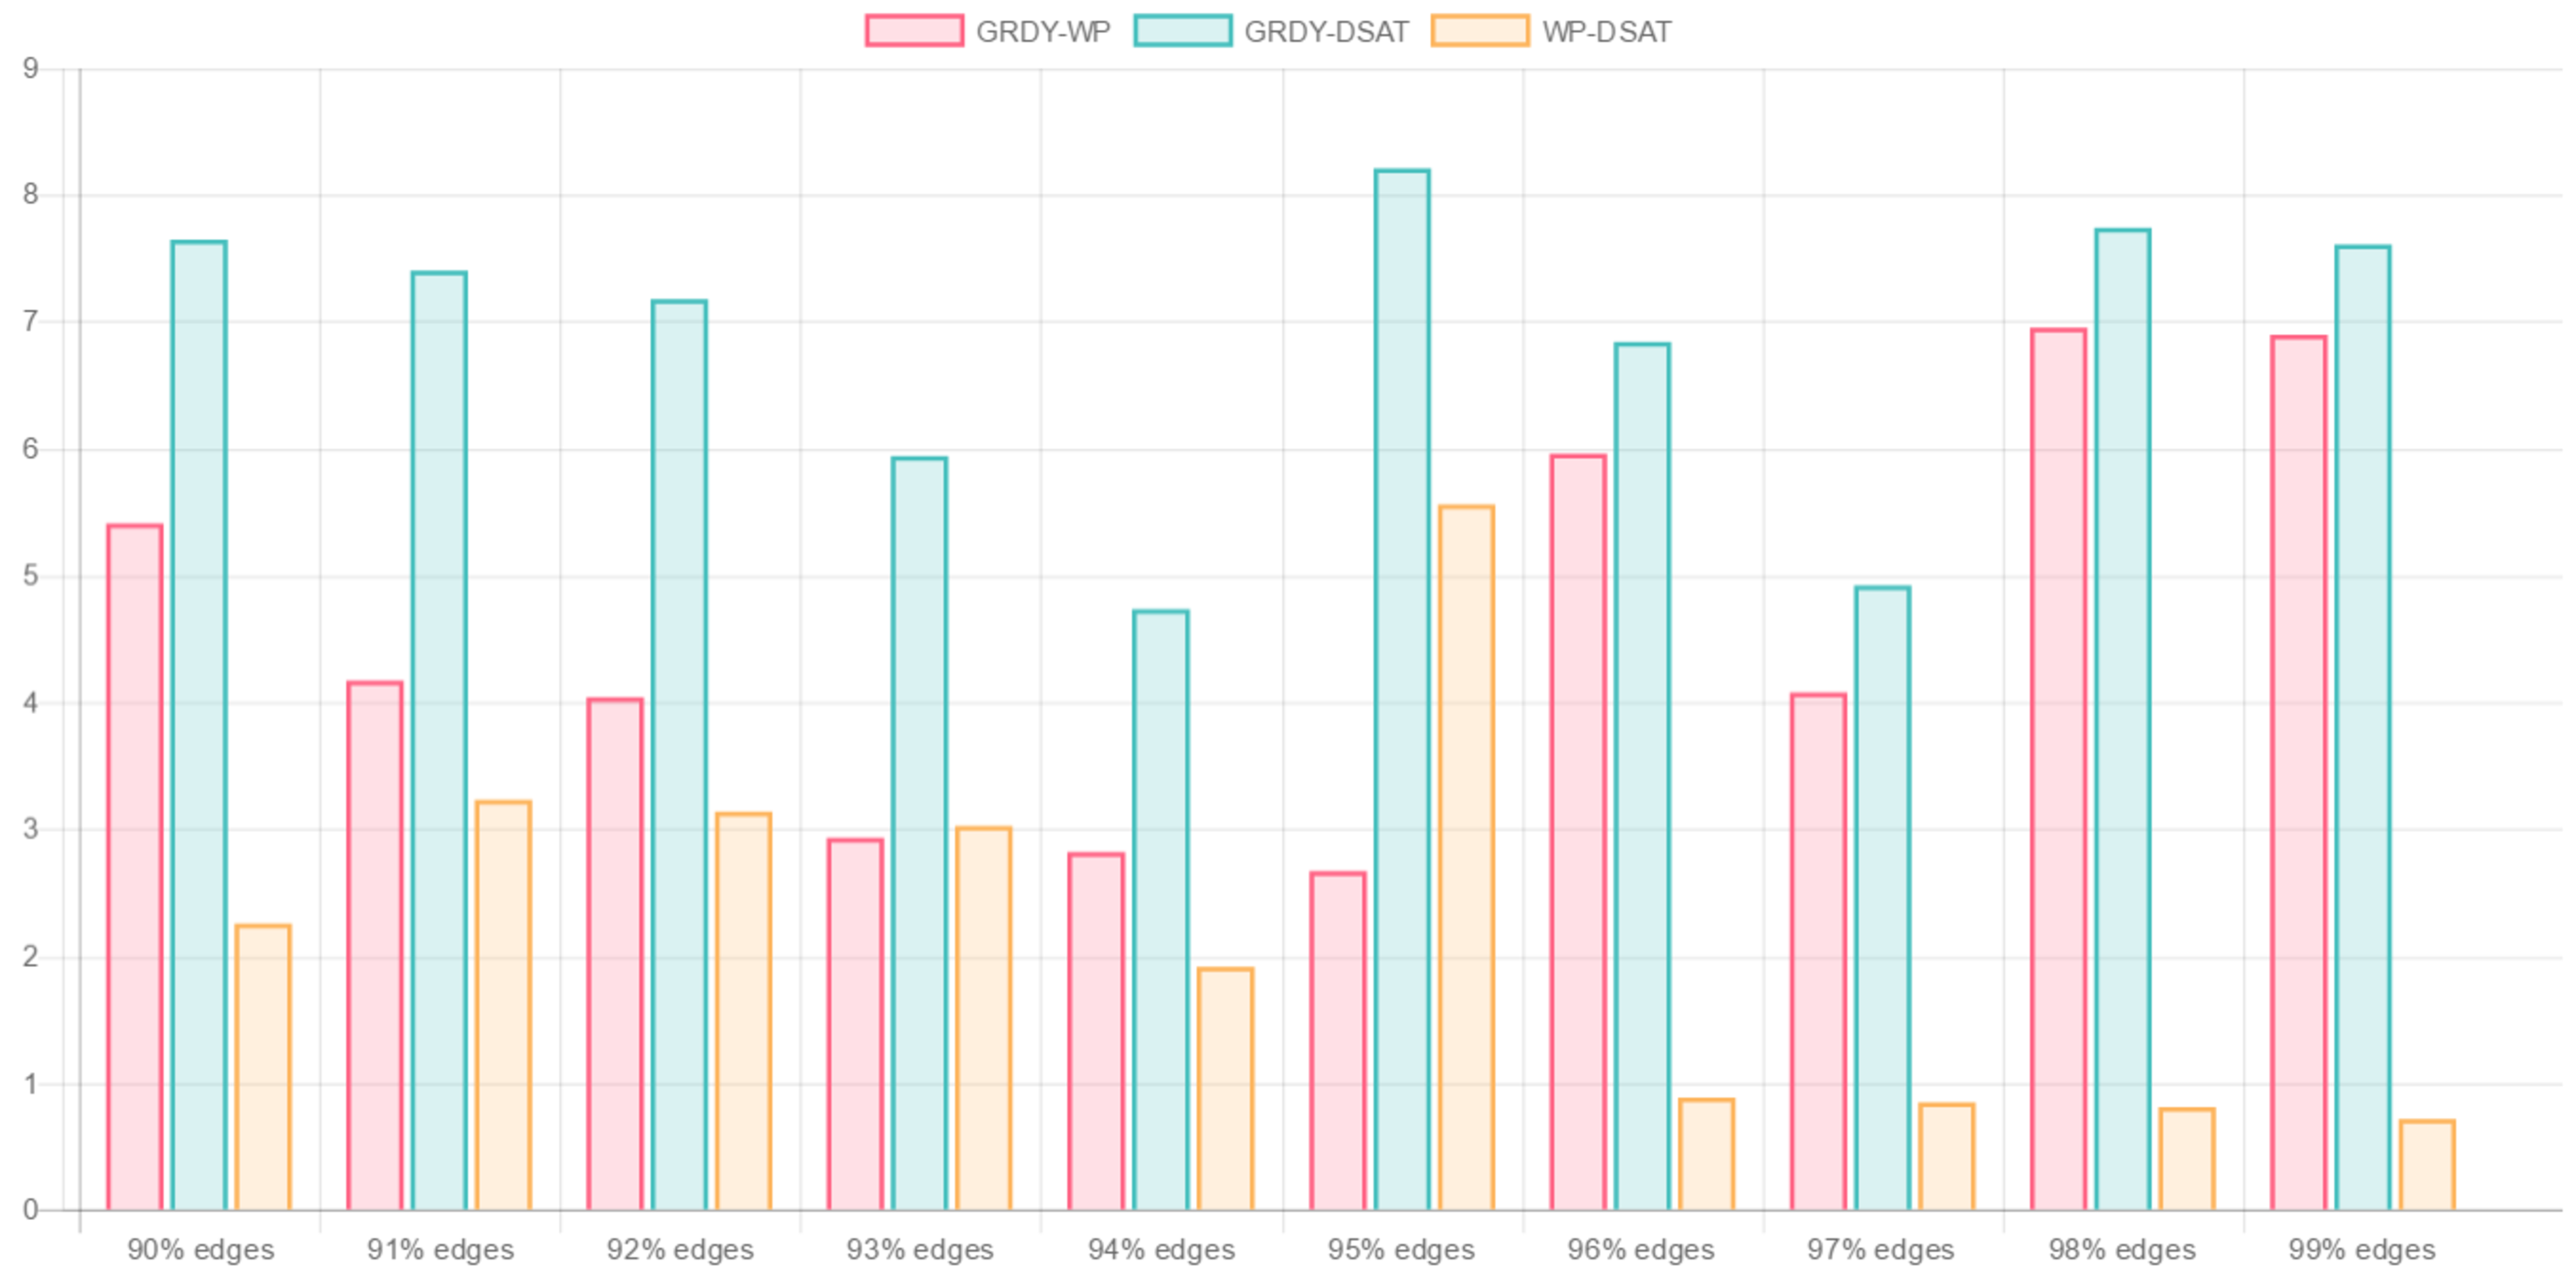
\includegraphics[width=\linewidth]{figures/comparison1-250.pdf}
            \caption{Percent difference of average colors used for 250 vertices}\label{fig:compare-250}
          \end{figure}
          \begin{figure}
            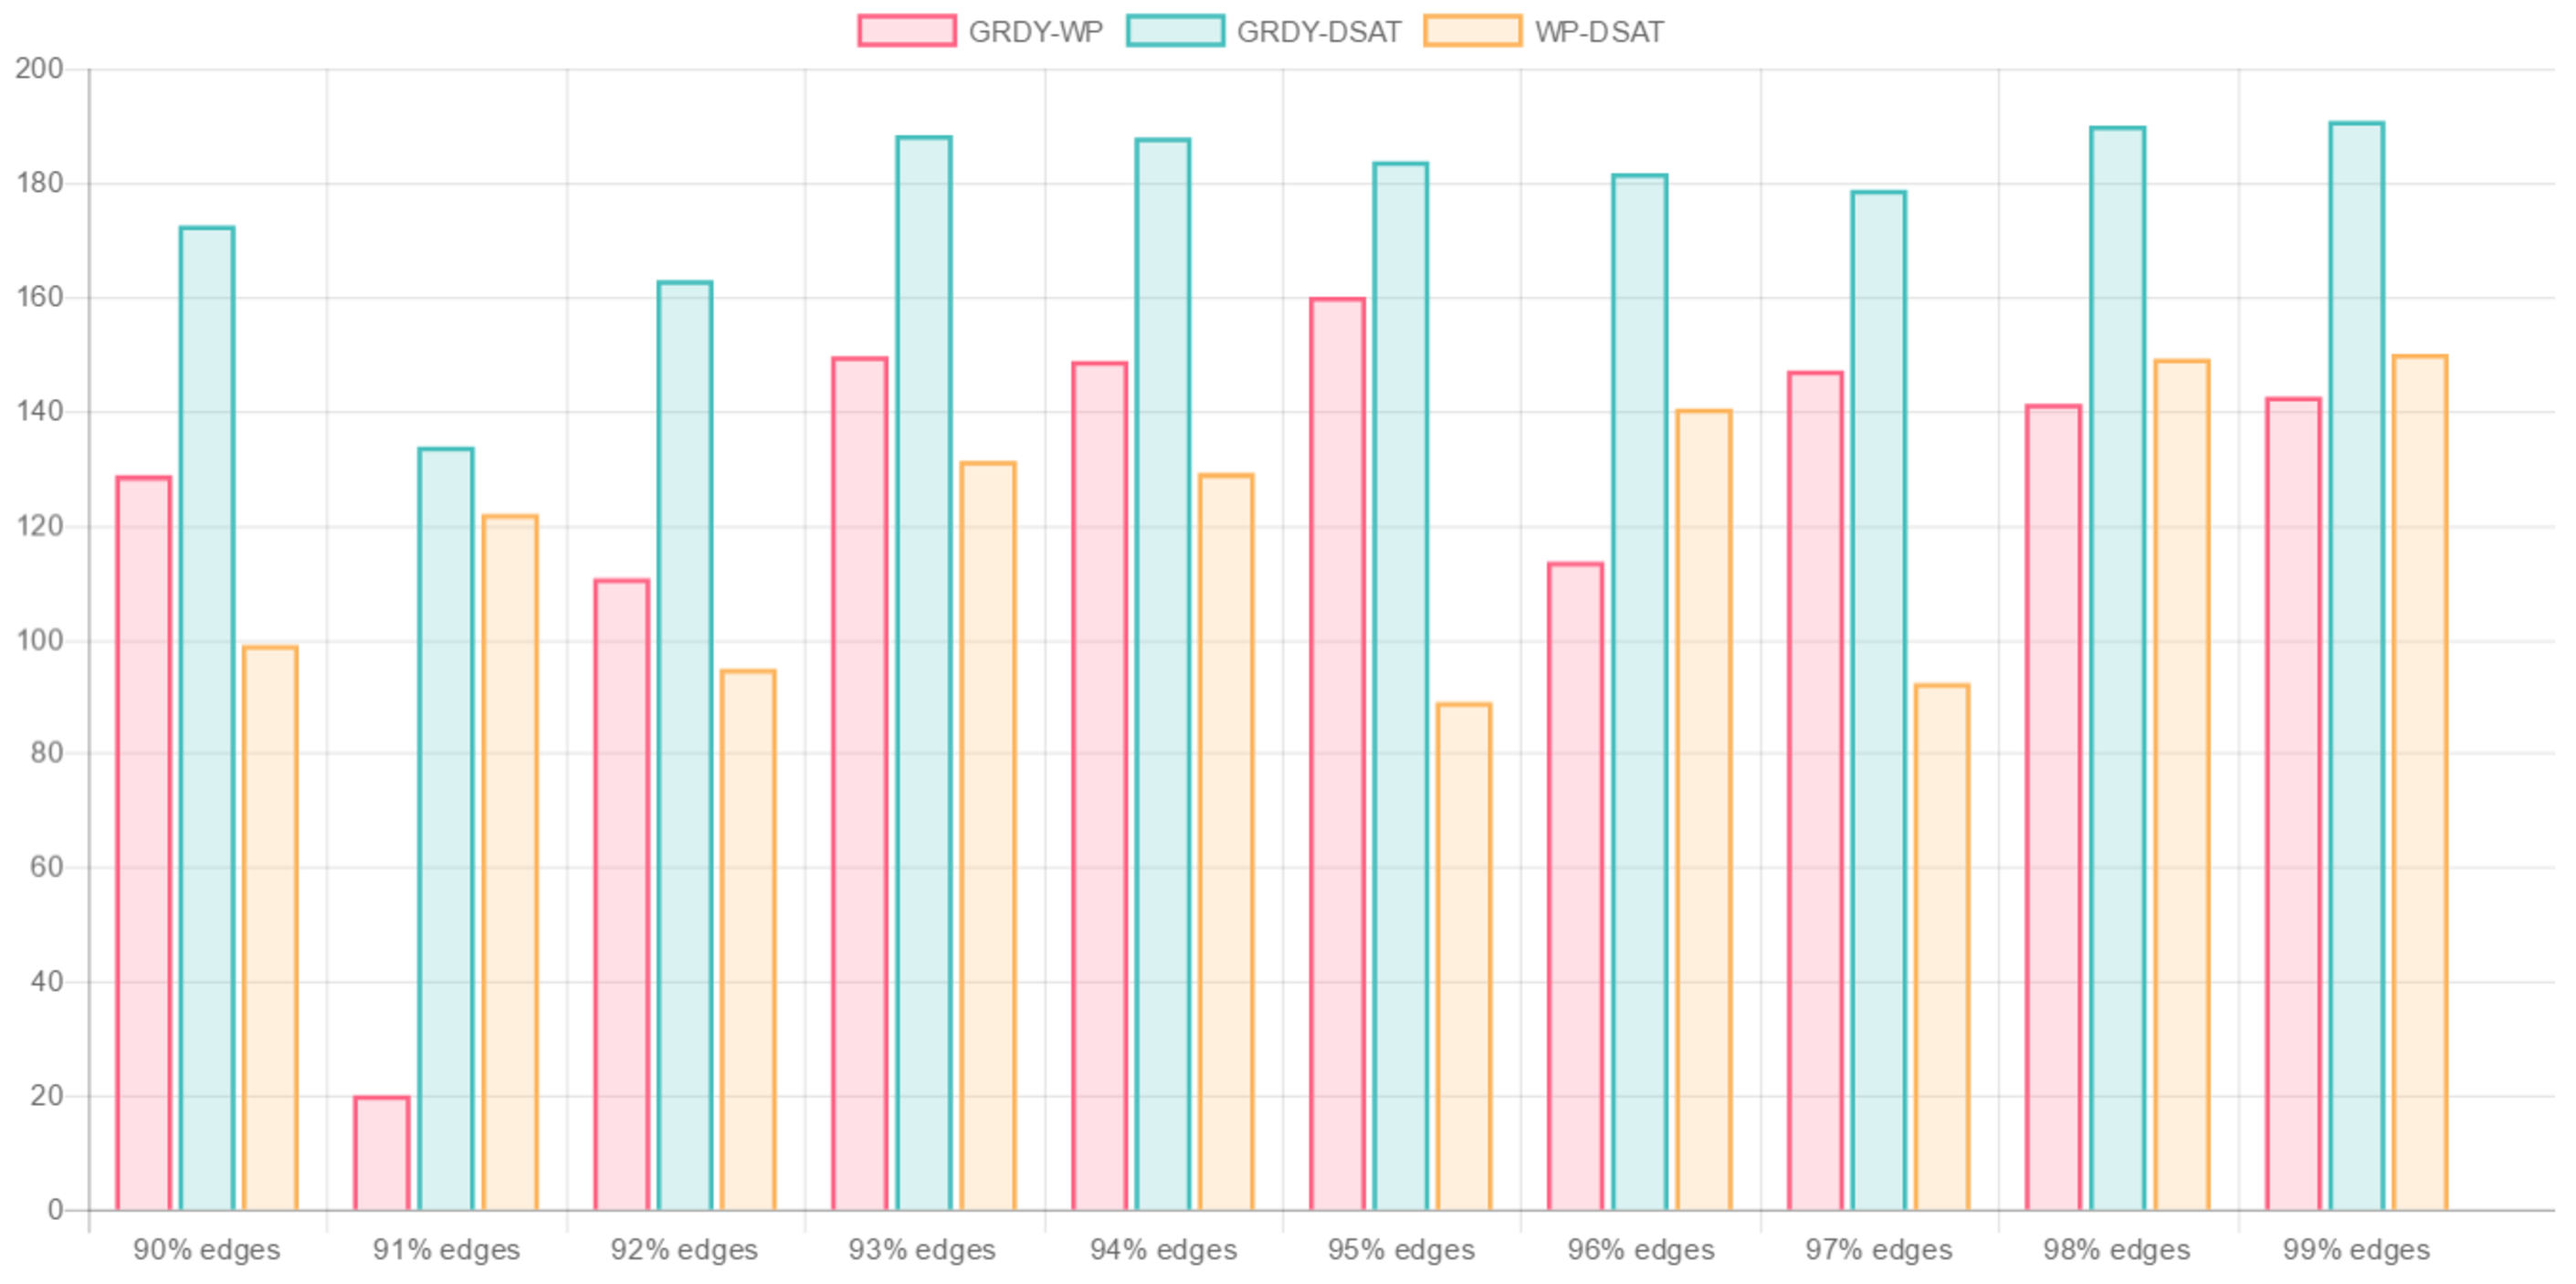
\includegraphics[width=\linewidth]{figures/comparison3-250.pdf}
            \caption{Percent difference of running time for 250 vertices}\label{fig:compare-time-250}
          \end{figure}
        \end{column}

      \end{columns}
    \end{block}

  \end{column}
  \begin{column}{\sepwid}\end{column}			% empty spacer column
  \begin{column}{\onecolwid}
    \vskip1.5ex

    \begin{figure}[h]
      \centering
      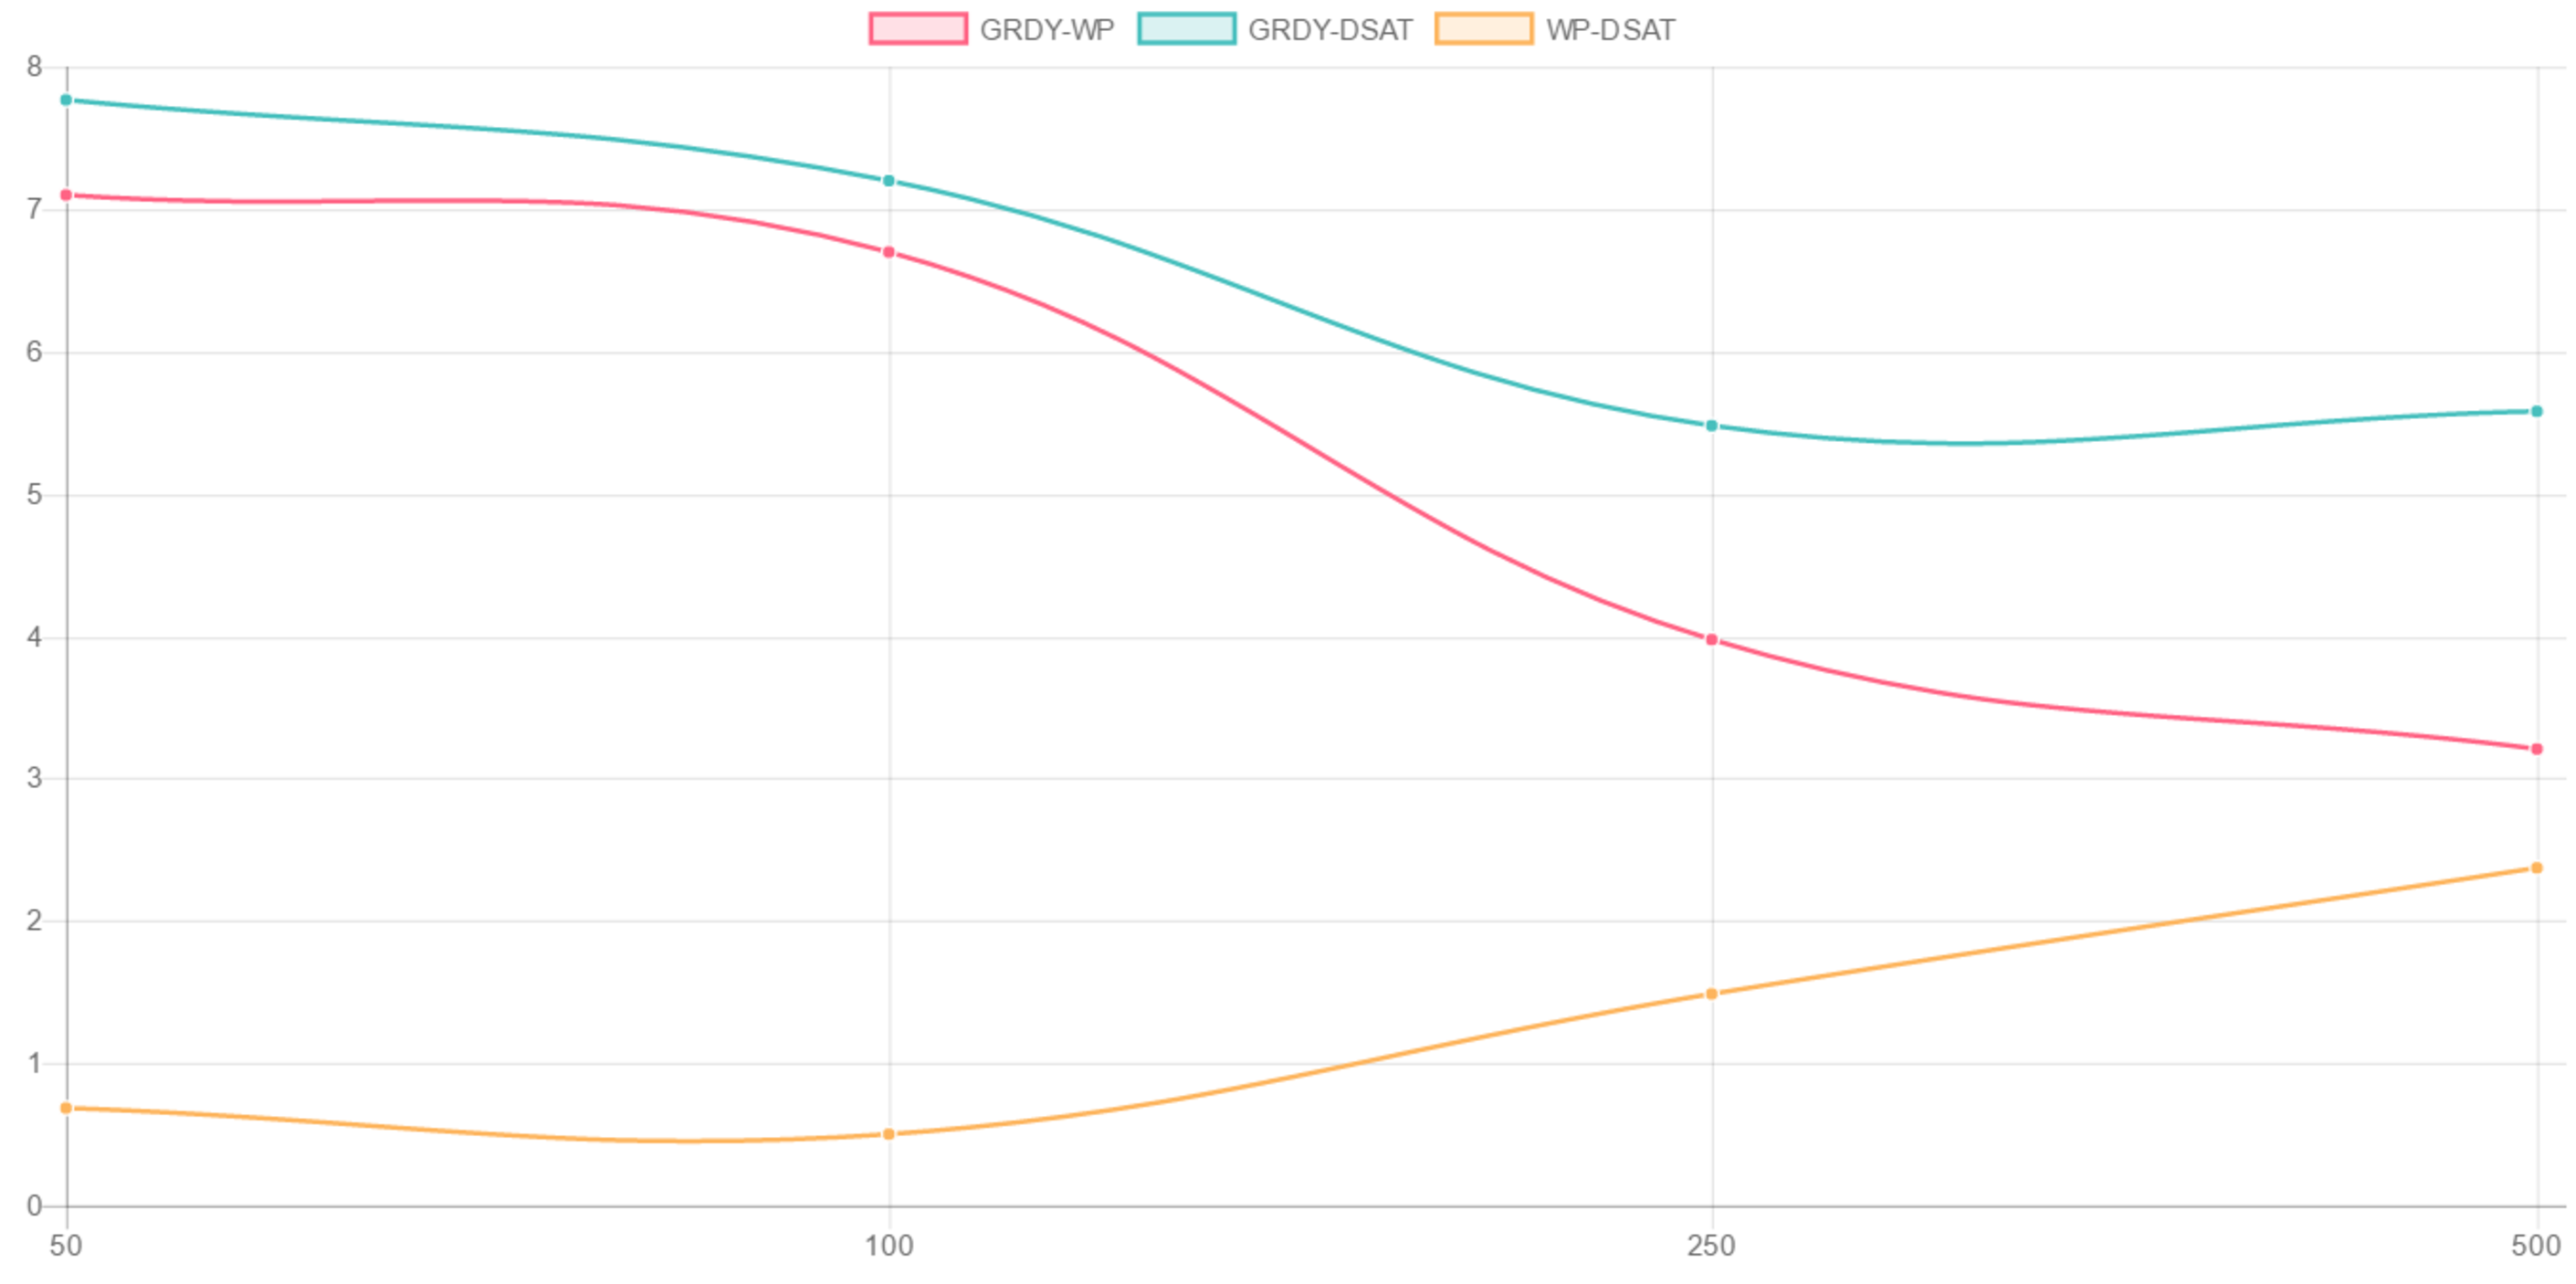
\includegraphics[width=\linewidth]{figures/comparison4.pdf}
      \caption{Percent difference of avg. colors used as vertices increase (93\% edges)}\label{fig:compare-min-250}
    \end{figure}

    \vspace{-0.2cm}

    \begin{itemize}
      \setlength\itemsep{0.4em}
      \rmfamily
      \item As the number of vertices increased, the percent difference between Greedy and Welsh-Powell as well as Greedy and DSATUR decreased. We also noticed that the percent difference between Welsh-Powell and DSATUR increased. This is shown in Figure \ref{fig:compare-min-250}.
      \item By looking at our comparisons, we saw that there is a \emph{partial order}.
      \begin{itemize}
        \item Welsh-Powell on average used $4-5\%$ less colors than Greedy.
        \item DSATUR on average used $6-7\%$ less colors than Greedy.
        \item DSATUR on average used $1-2\%$ less colors than Welsh-Powell.
      \end{itemize}
      \item This comparison stayed consistent when we looked at both minimum and maximum number of colors used.
      \item This led us to the following partial order based on colors used:
      \vspace{0.1cm}
      \begin{center}
        \textbf{Greedy $\leq$ Welsh-Powell $\leq$ DSATUR}
      \end{center}
      \item By looking at our running time comparisons, we saw:
      \begin{itemize}
        \item Welsh-Powell on average was $90-110\%$ slower than Greedy.
        \item DSATUR on average was $160-180\%$ slower than Greedy.
        \item DSATUR on average was $80-100\%$ slower than Welsh-Powell.
      \end{itemize}
    \end{itemize}

    \begin{block}{Conclusion}
      \begin{itemize}
        \item Although we were not able to compare the heuristics colorings to the optimal coloring, we were able to determine what heuristics gave the closest to optimal colors.
        \item Based on our results, we would suggest using the Welsh-Powell heuristic on most graphs.
        \begin{itemize}
          \item We decided that it would be worth 90-100\% more time to use 4-5\% less colors over Greedy. As most of these simulations ran in seconds, it is worth it.
          \item we decided it is \emph{not} worth using another 80-100\% more time to only use 1-2\% less colors if we use DSATUR over Welsh-Powell.
        \end{itemize}
      \end{itemize}
    \end{block}

    \begin{block}{References}
      %footnotesize
      \small{\rmfamily{\begin{thebibliography}{99}
      \setlength\parskip{0em}
      \setlength\itemsep{0em}

        \bibitem{bondymurty}
        Bondy, J.A. and U.S.R. Murty [1976],
        \emph{Graph theory with applications},
        American Elsevier Publishing, New York, NY.
        \bibitem{brelaz}
        Brélaz, D. [1979]. \emph{New methods to color the vertices of a graph}. Communications of the ACM, 22(4), pp.251-256.
        \bibitem{sharma}
        Sharma, P. C. and Chaudhari, N.S. [2012], \emph{A new reduction from 3-SAT to graph k-colorability for frequency assignment problem}, Int. J. Comp. Applic, 23-27.
        \bibitem{welsh}
        Welsh, D. J. and Powell, M. B. [1967], \emph{An upper bound for the chromatic number of a graph and its application to timetabling problems}, The Computer Journal, 10(1), 85-86.
      \end{thebibliography}}}
    \end{block}

  \end{column}
  \begin{column}{\sepwid}\end{column}			% empty spacer column
 \end{columns}
\end{frame}
\end{document}
